% Options for packages loaded elsewhere
\PassOptionsToPackage{unicode}{hyperref}
\PassOptionsToPackage{hyphens}{url}
%
\documentclass[
  12pt,
]{article}
\usepackage{amsmath,amssymb}
\usepackage{iftex}
\ifPDFTeX
  \usepackage[T1]{fontenc}
  \usepackage[utf8]{inputenc}
  \usepackage{textcomp} % provide euro and other symbols
\else % if luatex or xetex
  \usepackage{unicode-math} % this also loads fontspec
  \defaultfontfeatures{Scale=MatchLowercase}
  \defaultfontfeatures[\rmfamily]{Ligatures=TeX,Scale=1}
\fi
\usepackage{lmodern}
\ifPDFTeX\else
  % xetex/luatex font selection
\fi
% Use upquote if available, for straight quotes in verbatim environments
\IfFileExists{upquote.sty}{\usepackage{upquote}}{}
\IfFileExists{microtype.sty}{% use microtype if available
  \usepackage[]{microtype}
  \UseMicrotypeSet[protrusion]{basicmath} % disable protrusion for tt fonts
}{}
\makeatletter
\@ifundefined{KOMAClassName}{% if non-KOMA class
  \IfFileExists{parskip.sty}{%
    \usepackage{parskip}
  }{% else
    \setlength{\parindent}{0pt}
    \setlength{\parskip}{6pt plus 2pt minus 1pt}}
}{% if KOMA class
  \KOMAoptions{parskip=half}}
\makeatother
\usepackage{xcolor}
\usepackage[a4paper]{geometry}
\usepackage{color}
\usepackage{fancyvrb}
\newcommand{\VerbBar}{|}
\newcommand{\VERB}{\Verb[commandchars=\\\{\}]}
\DefineVerbatimEnvironment{Highlighting}{Verbatim}{commandchars=\\\{\}}
% Add ',fontsize=\small' for more characters per line
\usepackage{framed}
\definecolor{shadecolor}{RGB}{248,248,248}
\newenvironment{Shaded}{\begin{snugshade}}{\end{snugshade}}
\newcommand{\AlertTok}[1]{\textcolor[rgb]{0.94,0.16,0.16}{#1}}
\newcommand{\AnnotationTok}[1]{\textcolor[rgb]{0.56,0.35,0.01}{\textbf{\textit{#1}}}}
\newcommand{\AttributeTok}[1]{\textcolor[rgb]{0.13,0.29,0.53}{#1}}
\newcommand{\BaseNTok}[1]{\textcolor[rgb]{0.00,0.00,0.81}{#1}}
\newcommand{\BuiltInTok}[1]{#1}
\newcommand{\CharTok}[1]{\textcolor[rgb]{0.31,0.60,0.02}{#1}}
\newcommand{\CommentTok}[1]{\textcolor[rgb]{0.56,0.35,0.01}{\textit{#1}}}
\newcommand{\CommentVarTok}[1]{\textcolor[rgb]{0.56,0.35,0.01}{\textbf{\textit{#1}}}}
\newcommand{\ConstantTok}[1]{\textcolor[rgb]{0.56,0.35,0.01}{#1}}
\newcommand{\ControlFlowTok}[1]{\textcolor[rgb]{0.13,0.29,0.53}{\textbf{#1}}}
\newcommand{\DataTypeTok}[1]{\textcolor[rgb]{0.13,0.29,0.53}{#1}}
\newcommand{\DecValTok}[1]{\textcolor[rgb]{0.00,0.00,0.81}{#1}}
\newcommand{\DocumentationTok}[1]{\textcolor[rgb]{0.56,0.35,0.01}{\textbf{\textit{#1}}}}
\newcommand{\ErrorTok}[1]{\textcolor[rgb]{0.64,0.00,0.00}{\textbf{#1}}}
\newcommand{\ExtensionTok}[1]{#1}
\newcommand{\FloatTok}[1]{\textcolor[rgb]{0.00,0.00,0.81}{#1}}
\newcommand{\FunctionTok}[1]{\textcolor[rgb]{0.13,0.29,0.53}{\textbf{#1}}}
\newcommand{\ImportTok}[1]{#1}
\newcommand{\InformationTok}[1]{\textcolor[rgb]{0.56,0.35,0.01}{\textbf{\textit{#1}}}}
\newcommand{\KeywordTok}[1]{\textcolor[rgb]{0.13,0.29,0.53}{\textbf{#1}}}
\newcommand{\NormalTok}[1]{#1}
\newcommand{\OperatorTok}[1]{\textcolor[rgb]{0.81,0.36,0.00}{\textbf{#1}}}
\newcommand{\OtherTok}[1]{\textcolor[rgb]{0.56,0.35,0.01}{#1}}
\newcommand{\PreprocessorTok}[1]{\textcolor[rgb]{0.56,0.35,0.01}{\textit{#1}}}
\newcommand{\RegionMarkerTok}[1]{#1}
\newcommand{\SpecialCharTok}[1]{\textcolor[rgb]{0.81,0.36,0.00}{\textbf{#1}}}
\newcommand{\SpecialStringTok}[1]{\textcolor[rgb]{0.31,0.60,0.02}{#1}}
\newcommand{\StringTok}[1]{\textcolor[rgb]{0.31,0.60,0.02}{#1}}
\newcommand{\VariableTok}[1]{\textcolor[rgb]{0.00,0.00,0.00}{#1}}
\newcommand{\VerbatimStringTok}[1]{\textcolor[rgb]{0.31,0.60,0.02}{#1}}
\newcommand{\WarningTok}[1]{\textcolor[rgb]{0.56,0.35,0.01}{\textbf{\textit{#1}}}}
\usepackage{graphicx}
\makeatletter
\def\maxwidth{\ifdim\Gin@nat@width>\linewidth\linewidth\else\Gin@nat@width\fi}
\def\maxheight{\ifdim\Gin@nat@height>\textheight\textheight\else\Gin@nat@height\fi}
\makeatother
% Scale images if necessary, so that they will not overflow the page
% margins by default, and it is still possible to overwrite the defaults
% using explicit options in \includegraphics[width, height, ...]{}
\setkeys{Gin}{width=\maxwidth,height=\maxheight,keepaspectratio}
% Set default figure placement to htbp
\makeatletter
\def\fps@figure{htbp}
\makeatother
\setlength{\emergencystretch}{3em} % prevent overfull lines
\providecommand{\tightlist}{%
  \setlength{\itemsep}{0pt}\setlength{\parskip}{0pt}}
\setcounter{secnumdepth}{5}
\usepackage{fancyhdr}
\pagestyle{fancy}
\fancyhead{}
\fancyhead[R]{\small 2025-02-21}
\fancyhead[L]{\small Regression Linéaire}
\renewcommand{\headrulewidth}{0.4pt}
\ifLuaTeX
  \usepackage{selnolig}  % disable illegal ligatures
\fi
\usepackage{bookmark}
\IfFileExists{xurl.sty}{\usepackage{xurl}}{} % add URL line breaks if available
\urlstyle{same}
\hypersetup{
  pdfauthor={Dimitri DELPECH,; Timothé FADENIPO,; Matthis ARVOIS,; Ismael MADOU GAGI GREMA,; Cheikh LO},
  hidelinks,
  pdfcreator={LaTeX via pandoc}}

\title{\fbox{\huge Regression Linéaire}}
\author{Dimitri DELPECH, \and Timothé FADENIPO, \and Matthis
ARVOIS, \and Ismael MADOU GAGI GREMA, \and Cheikh LO}
\date{2025-02-21}

\begin{document}
\maketitle

{
\setcounter{tocdepth}{2}
\tableofcontents
}
\newpage

\section{Introduction}\label{introduction}

(en cours)

\section{Revue empirique}\label{revue-empirique}

La résistance du béton est une propriété reconnue depuis longtemps. Si
le béton est un élément important du développement de nos sociétés,
c'est qu'il possède une résistance mécanique, en particulier à la
compression, qui a permis aux architectes et concepteurs de concevoir
des structures de plus en plus importantes et durables dans le temps. La
propriété de la résistance du béton reste la propriété la plus
importante du matériau pour du point de vue de l'ingénieur. Depuis
longtemps, la relation entre la composition du béton et la résistance au
béton fait écho dans le monde du génie civil et intéresse de nombreux
chercheurs de ce domaine. Cependant aucune théorie fondamentale et
universellement adoptée n'existe, en la matière, au-delà de la notion
commune de rapport eau/ciment. Cette première partie a pour but de
mettre en lumière les effets des variables explicatives sur la variable
cible en l'occurrence sur la résistance à la compression du béton en se
basant sur les travaux effectués dans ce sens.

Bien que dans toute approche fondamentale de la résistance à la
compression, la nature du granulat représente un rôle secondaire
néanmoins ceci reste important pour notre étude. Dans les années 1960,
Walker et Bloem ont publié dans leur article (Effect of Aggregate size
on properties of concrete, journal of AIC,septembre) un résultat assez
percutant. Il s'agit de la démonstration de l'effet négatif du volume de
la dimension maximale sur la résistance. Trois effets du granulat sur la
résistance du béton ont été énumérés à savoir un effet d'adhérence ;
l'effet de confinement et l'effet plafond (le Bulletin des Laboratoires
des Ponts et Chaussées, numéro 219, en janvier-février 1999, pages 41 à
52.).

A part son rôle important dans le phénomène de l'hydratation, l'eau est
l'un des facteurs les plus importants au niveau de l'ouvrabilité du
béton. L'augmentation du dosage en eau augmente la fluidité du béton et
entraîne la diminution de la concentration en solides. Cependant,
l'introduction excessive de l'eau provoque la chute de la résistance
mécanique et sa durabilité (effect on composition parameters on fresh
state properties of self-compacting concrete N.Bouhamou et al.). Le
bulletin publié par FEBELCEM (Fédération de l'Industrie Cimentière
Belge) avec l'auteur Ir C.Ployaert que la durabilité d'un béton dépend
d'une faible porosité. De plus, pour les surfaces de bétonnage non
coffrées sont les plus critiques du fait de leur exposition au soleil et
au vent. Le contrôle de leur protection efficace contre toute
évaporation intempestive de l'eau nécessaire à l'hydratation du ciment
revêt d'une grande importance. D'où la liaison importante entre la
résistance à la compression et l'eau.

Puis dans l'article publié par le département de génie civil à
l'université de Mostaganem en Algérie, le rôle de superplastifiant a été
mis en exergue. Le volume d'eau augmente avec l'augmentation du dosage
en superplastifiant. L'une des explications avancées est l'augmentation
de la viscosité de l'eau due au superplastifiant. De plus, il est noté
que l'augmentation du dosage en superplastifiant a engendré une
augmentation du taux de ségrégation statique dans le cas où le dosage
est élevé entraînant ainsi une réduction de l'homogénéité du béton et
par conséquent une réduction sa résistance à la compression. Par
ailleurs, un dosage modéré en superplastifiants apporte un bénéfice
supplémentaire, particulièrement aux premiers âges (48h, 72h), en raison
d'une meilleure compacité et d'une dispersion plus efficace des grains
de ciment.

Ensuite, Mehta et Monteiro (2014) soulignent que l'augmentation de la
teneur en ciment améliore significativement la résistance mécanique, en
particulier dans les premiers jours de durcissement. De même, Siddique
et al.~(2011) ont observé une corrélation positive entre la teneur en
ciment et la résistance à la compression, confirmant que cette relation
est particulièrement marquée dans les premières phases de durcissement.
Toutefois, au-delà d'un certain seuil, une concentration excessive de
ciment peut entraîner des effets négatifs, notamment une élévation de la
chaleur d'hydratation et une augmentation du retrait, favorisant ainsi
l'apparition de fissures (Neville, 2011). Il a également spécifié qu'il
existe une diminution dans l'efficacité du ciment en appliquant de très
haut dosage même en présence de superplastifiant dans ADDIS B.J ,
Alexandre M.G (1994) . Le dosage du ciment dans le béton est très
souvent relié à ses propriétés mécaniques et sa durabilité (effect on
composition parameters on fresh state properties of self-compacting
concrete N.Bouhamou et al.).

Par ailleurs, le laitier de haut fourneau est souvent utilisé pour
remplacer une partie du ciment afin d'améliorer certaines propriétés du
béton. Plusieurs études ont montré que son ajout réduit la résistance du
béton dans les premiers jours, car sa réaction est plus lente que celle
du ciment classique. Cependant, à plus long terme, il aide à renforcer
le béton grâce à une réaction chimique qui produit des éléments solides
supplémentaires, améliorant ainsi sa résistance (Jin et al., 2003).

De plus, l'utilisation des cendres volantes pour remplacer une partie du
ciment a aussi un impact sur la résistance du béton. D'après Tan et
al.~(2016), leur ajout réduit la résistance dans les premiers jours, car
elles réagissent plus lentement que le ciment. Toutefois, avec le temps,
elles renforcent la structure du béton et améliorent sa durabilité grâce
à une réaction chimique progressive. Zhao et al.~(2019) précisent que
leur effet dépend de la quantité utilisée et de la finesse des
particules, ce qui influence directement la résistance finale du béton.

En outre, Les granulats fins, communément appelés ``Fine Aggregate'',
constituent la fraction sableuse dans la formulation du béton. On
considère généralement qu'il s'agit de particules de dimensions
inférieures à 5 mm. La quantité de granulats fins, principalement
constitués de sable, influence la résistance du béton. Selon Chatterji
(2013), une bonne proportion de granulats fins améliore la compacité du
mélange, réduit la porosité et augmente la résistance à la compression.
Cependant, un excès de sable peut affaiblir la structure en diminuant la
cohésion entre les particules de ciment et les granulats plus gros
(Neville, 2011). Concrètement, une teneur adéquate en sable améliore le
contact entre la pâte cimentaire et les grains, réduisant la porosité et
favorisant ainsi un meilleur transfert des contraintes. Il est donc
essentiel de trouver un équilibre pour garantir une répartition homogène
des matériaux et optimiser la résistance du béton. Quant à l'étude du
bulletin des laboratoires des ponts et chaussées (1999) intitulée
``Influence du granulat sur la résistance à la compression des bétons'',
elle révèle qu'entre 60 \% et 75 \% de volume total d'agrégats, une
variation de la proportion de granulats fins peut entraîner un écart de
l'ordre de 2 à 3 MPa en résistance à la compression. La raison tient à
la formation d'une couche de pâte cimentaire plus ou moins épaisse selon
la quantité de sables incorporée, conditionnant ainsi la compacité et la
performance mécanique du béton. Enfin, L'âge du béton (Age) se définit
comme la durée écoulée depuis le coulage et le compactage jusqu'à la
réalisation des essais mécaniques, habituellement exprimée en nombre de
jours (1, 2, 7, 28, etc.). Il revêt une grande importance, car plus le
béton mûrit, plus la réaction d'hydratation du ciment se poursuit,
consolidant la microstructure et augmentant de manière significative la
résistance en compression. Plusieurs études, dont celles de Neville
(2011), Mindess et Young (2019), montrent que la résistance du béton
augmente avec le temps en raison du processus d'hydratation du ciment.
La majeure partie du gain de résistance se produit au cours des 28
premiers jours, période pendant laquelle le ciment continue de réagir
avec l'eau pour former une structure solide. Cependant, le taux de
durcissement ralentit après cette période, bien que certaines
formulations, notamment celles contenant du laitier ou des cendres
volantes, puissent encore voir leur résistance s'améliorer au-delà de 90
jours. Selon les observations présentées dans un mémoire de recherche
intitulé ``Impact du superplastifiant sur les propriétés
physico-mécaniques du ciment'' à l'université de Blida 1(2022-2023), la
résistance à la compression connaît une croissance rapide entre 1 et 7
jours, passant de 20 \% de la résistance ultime à près de 70 \% autour
de la première semaine . Typiquement, un saut d'environ 10 MPa (environ
50 \%) est constaté entre 2 et 7 jours. Après ce cap, le rythme de
durcissement ralentit, mais on atteint souvent plus de 90 \% de la
résistance finale à 28 jours. \# Analyse univariée.

\subsection{Première variable.}\label{premiuxe8re-variable.}

La variable qui répertorie les résistances à la compression des bétons
étudiés, que nous avons choisi d'expliquer grâce aux autres, est bien
distribuée, sans valeurs aberrantes, avec des résistances variant entre
2 MPa (mégapascals) et 80 MPa, pour une moyenne et une médiane autour de
35 MPa. Cette bonne distribution nous sera utile pour la suite de
l'étude.

\subsection{Suite}\label{suite}

Variable resistance du beton(``y\_concrete\_compresive'') :

Variable (``fine\_aggr'') :

Variable eau (``Water''):

les variable sont principalements concentrés autour de la médiane ce qui
pourrait indiquer par exemple pour la variable de resitance du beton que
la plupart des échantillons de béton ont une résistance similaire

Variable cendre volante(``fly\_ash''):

Variable Quantité de laitier(``blast\_furnace''):

Variable cendre volante(``fly\_ash''):

Variable superplastique(``super\_plast''):

Ces variables sont fortements concentrés surdes données faibles et
minimales

\section{Analyse bivariée.}\label{analyse-bivariuxe9e.}

La matrice de corrélation en annexe va nous aider à voir les différents
liens de corrélation potentiels entre nos variables. Dans cette partie,
nous allons étudier et essayer de trouver les couples de variables
significativement dépendants. Il est important de trouver tous les
couples liés afin d'expliquer de manière optimale comment les variables
de notre base peuvent influer sur la résistance à la compression du
béton.

\subsection{Quantité de ciment et résistance du
béton.}\label{quantituxe9-de-ciment-et-ruxe9sistance-du-buxe9ton.}

Nous allons ici examiner si la quantité de ciment utilisée pour créer le
béton est significativement reliée à la résistance à la compression du
béton. En effet, nous pouvons d'abord observer la distribution de ces
deux variables à l'aide du graphique ci-dessous :

\begin{center}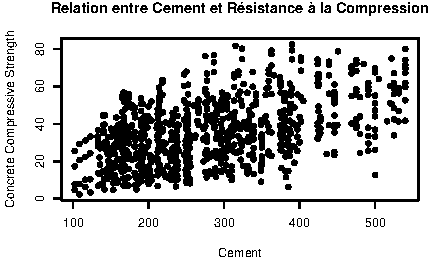
\includegraphics{rmd_final_files/figure-latex/unnamed-chunk-2-1} \end{center}

Cette visualisation des données nous donne une première impression du
lien potentiel entre ces deux variables. En étudiant plus précisément
ces deux variables avec un test de corrélation de Pearson, on se rend
compte qu'il y a un lien significatif : ces deux variables sont
positivement liées.

On peut alors dire que plus la quantité de ciment utilisée pour la
fabrication du béton est grande, plus la résistance à la compression de
ce béton sera importante. Le test final a donné un coefficient de
corrélation \(\rho\) de Pearson égal à \textbf{0,5} (annexe), ce qui
indique un lien relativement fort et non négligeable. Ainsi, une
fabrication de béton comprenant une grande quantité de ciment
favoriserait grandement sa résistance à la compression.

\subsection{Additif chimique et eau.}\label{additif-chimique-et-eau.}

Dans le processus de fabrication du béton, il est parfois nécessaire
d'ajouter un additif chimique pour améliorer sa fluidité et sa
maniabilité. La réflexion porte ici sur la corrélation entre l'ajout de
cet additif chimique et la quantité d'eau utilisée pour la fabrication :
y aurait-il un quelconque lien entre ces deux variables ?

Pour ce faire, il semble juste d'examiner les différents ajouts
d'additif en fonction de la quantité d'eau utilisée pour chaque béton.
Le graphique ci-dessous illustre cette relation, et nous pouvons
aisément supposer qu'il existe une corrélation entre ces deux variables.
En effet, dans l'ensemble, on remarque une diminution de l'ajout
d'additif lorsque la quantité d'eau augmente.

\begin{center}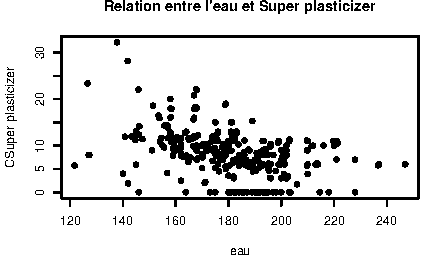
\includegraphics{rmd_final_files/figure-latex/unnamed-chunk-3-1} \end{center}

Pour avoir une certitude, nous effectuons alors un test de corrélation
de Kendall, qui nous indique, premièrement, qu'il existe un lien
significatif entre ces deux variables et, deuxièmement, que le
coefficient de corrélation \(\tau\) étant de \textbf{-0.53} (annexe), la
négativité de la liaison est prouvée.

En clair, plus la quantité d'eau utilisée pour la fabrication du béton
est importante, moins d'additif chimique a été ajouté lors de cette
fabrication. Ce lien fort nous aidera dans la suite de notre étude.

\subsection{L'age, une variable
importante.}\label{lage-une-variable-importante.}

Il serait tout à fait naturel de penser que l'âge ait une quelconque
importance sur la résistance à la compression du béton. En effet,
l'imaginaire collectif nous amène d'abord à penser que ce béton, en
conséquence de l'âge, deviendrait de plus en plus fragile et, de ce
fait, moins résistant à la compression. Notre hypothèse serait alors de
dire que l'âge est négativement lié à la résistance à la compression du
béton, \(i.e.\), plus l'âge augmente, moins le béton est résistant.

Dans un premier temps, l'observation de la distribution du temps par
rapport à la compression nous aiderait à confirmer ou infirmer
l'hypothèse de cette partie. Voyons le graphique ci-dessous.

\begin{center}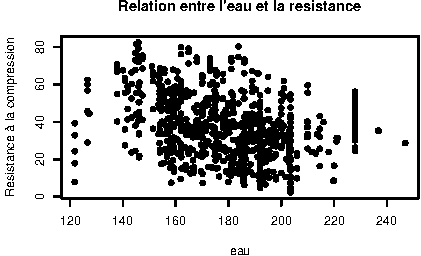
\includegraphics{rmd_final_files/figure-latex/unnamed-chunk-4-1} \end{center}

Cette première visualisation ne nous permet pas de dire s'il y aurait en
réalité un quelconque lien entre ces deux variables. En conséquence, il
est nécessaire de réaliser un test de corrélation.

Ici, le test réalisé nous permet de voir que notre hypothèse est
infirmée, car il y a en effet un lien significatif entre ces deux
variables, et la corrélation indique que ce lien est positif. Cette
corrélation est positive mais modérée, avec un coefficient de Kendall
\(\tau\) de \textbf{0,449} (annexe). Les valeurs croissent
significativement ensemble, mais il y aura tout de même quelques
exceptions.

\section{Analyse Multivariée}\label{analyse-multivariuxe9e}

Dans cette partie, nous allons étudier l'ensemble des variables en
utilisant une analyse en composantes principales (ACP). La variable à
expliquer (\texttt{y\_concrete\_compresive}) est placée en supplément,
tandis que les huit autres variables (les variables explicatives) sont
considérées comme actives dans l'ACP.

\subsection{Analyse en Composantes
Principales}\label{analyse-en-composantes-principales}

\begin{center}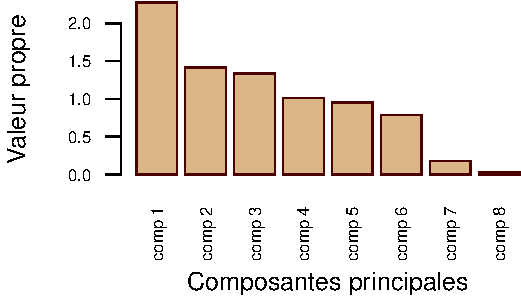
\includegraphics{rmd_final_files/figure-latex/unnamed-chunk-5-1} \end{center}

Le graphique illustre l'histogramme des valeurs propres issu de l'ACP,
permettant d'identifier combien d'axes principaux il est pertinent de
retenir.

\begin{itemize}
\tightlist
\item
  Le premier axe affiche une valeur propre autour de \textbf{2.0},
  indiquant qu'il concentre une part importante de la variance totale.
\item
  Le deuxième axe, avec une valeur propre avoisinant \textbf{1.5},
  conserve également une proportion significative d'information.
\item
  Les troisième et quatrième axes présentent des valeurs légèrement
  inférieures ajoutant encore un complément notable de variance.
\item
  À partir du cinquième axe, les valeurs propres décroissent nettement,
  indiquant une contribution plus marginale à la variabilité des
  données.
\end{itemize}

En appliquant la \textbf{règle du coude}, il est judicieux de retenir
les \textbf{deux ou trois premiers axes} pour une analyse plus
approfondie.

\subsection{Analyse sur les 2 Premiers
Axes}\label{analyse-sur-les-2-premiers-axes}

\begin{center}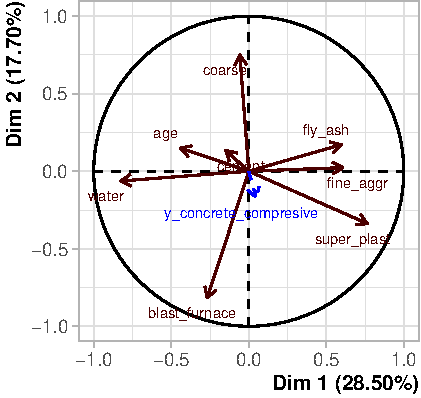
\includegraphics{rmd_final_files/figure-latex/unnamed-chunk-6-1} \end{center}

Le cercle de corrélation met en lumière les relations entre les
variables étudiées, projetées sur les deux premiers axes principaux de
l'ACP. Ces axes capturent ensemble \textbf{46,2 \%} de la variance
totale des données (\textbf{28,50 \% pour Dim 1 et 17,7 \% pour Dim 2}).

\subsubsection{Interprétation du Premier Axe (Dim 1 : 28,50
\%)}\label{interpruxe9tation-du-premier-axe-dim-1-2850}

Le premier axe oppose \textbf{la teneur en eau (\texttt{water}) et l'âge
du béton (\texttt{age})} aux formulations utilisant \textbf{des
superplastifiants (\texttt{super\_plast}), des cendres volantes
(\texttt{fly\_ash}) et une plus grande proportion de granulats fins
(\texttt{fine\_aggr})}.

\begin{itemize}
\tightlist
\item
  \texttt{water} (29,93 \% de contribution, cos² = 0.68) est la variable
  la plus représentée sur Dim 1.
\item
  \texttt{super\_plast} (25,59 \% de contribution, cos² = 0.58) est
  projeté dans la direction opposée à \texttt{water}. Cela traduit son
  rôle dans l'amélioration de la fluidité du béton et la réduction du
  besoin en eau, permettant une meilleure résistance.
\item
  \texttt{fly\_ash} (15,57 \% de contribution, cos² = 0.35) est bien
  projeté sur cet axe, montrant que l'incorporation de cendres volantes
  influence la résistance du béton.
\item
  \texttt{fine\_aggr} (16,15 \% de contribution, cos² = 0.37) est bien
  représenté sur Dim 1, indiquant que la proportion de granulats fins
  influence la maniabilité et la compacité du béton.
\item
  \texttt{age} (8,50 \% de contribution, cos² = 0.19) est aussi bien
  représenté sur Dim 1.
\item
  \texttt{y\_concrete\_compresive} est projetée dans la même direction
  que \texttt{super\_plast}, suggérant une corrélation avec une
  meilleure résistance finale, tandis qu'une forte teneur en eau
  (\texttt{water}) est corrélée négativement à la résistance.
\end{itemize}

\subsubsection{Interprétation du Deuxième Axe (Dim 2 : 17,7
\%)}\label{interpruxe9tation-du-deuxiuxe8me-axe-dim-2-177}

Le deuxième axe met en opposition \textbf{la quantité de laitier de haut
fourneau (\texttt{blast\_furnace}) et la quantité de granulats grossiers
(\texttt{coarse})}.

\begin{itemize}
\tightlist
\item
  \texttt{blast\_furnace} (47,01 \% de contribution, cos² = 0.66) est la
  variable la plus représentée sur Dim 2. Son influence montre que
  l'ajout de laitier de haut fourneau différencie certaines formulations
  de béton, influençant leur durabilité.
\item
  \texttt{coarse} (39,73 \% de contribution, cos² = 0.56) est également
  bien projeté sur Dim 2.
\end{itemize}

\subsection{Implications pour la Modélisation de la Résistance du
Béton}\label{implications-pour-la-moduxe9lisation-de-la-ruxe9sistance-du-buxe9ton}

\begin{itemize}
\tightlist
\item
  L'axe 1 montre une forte opposition entre \texttt{water} et
  \texttt{super\_plast}, indiquant qu'un \textbf{terme d'interaction}
  entre ces deux variables pourrait être testé dans notre modèle
  linéaire.
\item
  \texttt{fine\_aggr} étant bien projeté sur Dim 1, son interaction avec
  \texttt{super\_plast} pourrait être pertinente pour examiner leur
  effet combiné sur la compacité et la résistance.
\item
  \texttt{age} étant bien projeté sur Dim 1, son interaction avec
  \texttt{water} pourrait également être pertinente.
\item
  L'axe 2 suggère que l'interaction entre \texttt{blast\_furnace} et
  \texttt{coarse} pourrait être testée pour examiner leur influence
  combinée sur la résistance mécanique.
\end{itemize}

\subsection{Interprétation du Troisième
Axe}\label{interpruxe9tation-du-troisiuxe8me-axe}

\subsubsection{Dim(1-3) : 45 \% de la Variance
Totale}\label{dim1-3-45-de-la-variance-totale}

\begin{itemize}
\tightlist
\item
  \texttt{cement} est très bien représenté (cos² = 0.88) et contribue en
  grande partie à la construction de cet axe (66 \%).
\item
  \texttt{fly\_ash} contribue à hauteur de 17 \% à la construction de
  cet axe et est bien représenté avec cos² = 0.22.
\item
  \texttt{y\_concrete\_compresive} suit la même direction que
  \texttt{cement}, suggérant une influence positive sur la résistance à
  la compression.
\end{itemize}

\subsubsection{Dim(2-3) : 35 \% de la Variance
Totale}\label{dim2-3-35-de-la-variance-totale}

\begin{itemize}
\tightlist
\item
  Contrairement à la précédente interprétation, on remarque que
  \textbf{la combinaison de \texttt{cement} et \texttt{fly\_ash}
  augmente la résistance du béton}.
\item
  Ce contraste sera analysé plus précisément après la construction du
  modèle.
\end{itemize}

\subsection{Conclusion}\label{conclusion}

Cette ACP met en évidence trois dimensions principales dans la
composition du béton :

\begin{enumerate}
\def\labelenumi{\arabic{enumi}.}
\tightlist
\item
  \textbf{Axe 1 (Dim 1)} : Opposition entre l'eau et les
  superplastifiants, cendres volantes et granulats fins.
\item
  \textbf{Axe 2 (Dim 2)} : Opposition entre le laitier de haut fourneau
  et les granulats grossiers.
\item
  \textbf{Axe 3 (Dim 3)} : Influence du lien \texttt{cement-fly\_ash}
  sur la résistance à la compression du béton.
\end{enumerate}

\section{Regression .}\label{regression-.}

(lm(formula = , data = ).. + REGARDER Intercept + faire graphique +
regarder coeffs + retirer des variable a cause de l'analyse bivairée

\section{Conclusion}\label{conclusion-1}

\section{Annexe}\label{annexe}

\subsection{Analyse univariée}\label{analyse-univariuxe9e}

Boite à moustache pour la variable
\texttt{Concrete\ compressive\ strength}.

\begin{center}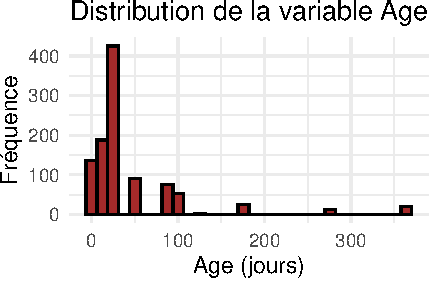
\includegraphics{rmd_final_files/figure-latex/unnamed-chunk-7-1} \end{center}

\subsection{Analyse bivariee}\label{analyse-bivariee}

Matrice de correlation

\begin{center}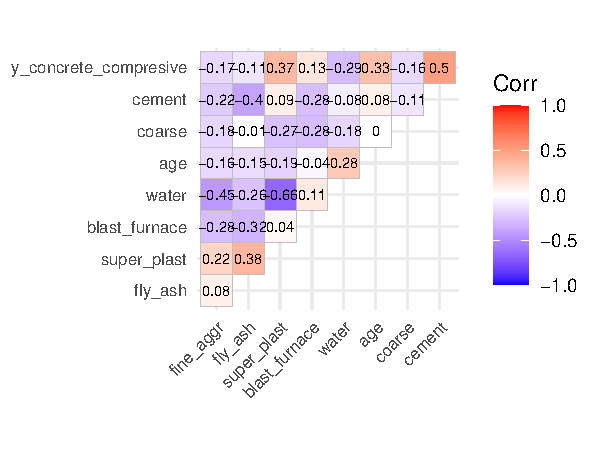
\includegraphics{rmd_final_files/figure-latex/corr_y-1} \end{center}

test corrrelation entre variable à expliquer et \texttt{cement}

\begin{Shaded}
\begin{Highlighting}[]
\FunctionTok{cor.test}\NormalTok{(bdd}\SpecialCharTok{$}\NormalTok{cement, bdd}\SpecialCharTok{$}\NormalTok{y\_concrete\_compresive, }\AttributeTok{method =} \StringTok{"pearson"}\NormalTok{)}
\end{Highlighting}
\end{Shaded}

\begin{verbatim}
## 
##  Pearson's product-moment correlation
## 
## data:  bdd$cement and bdd$y_concrete_compresive
## t = 18.405, df = 1028, p-value < 2.2e-16
## alternative hypothesis: true correlation is not equal to 0
## 95 percent confidence interval:
##  0.4504473 0.5424213
## sample estimates:
##       cor 
## 0.4978327
\end{verbatim}

\begin{Shaded}
\begin{Highlighting}[]
\CommentTok{\#test de pearson car ont une distribution pseudo{-}normale}
\end{Highlighting}
\end{Shaded}

test de correlation entre variable \texttt{water} et
\texttt{SuperPlasticizer}

\begin{Shaded}
\begin{Highlighting}[]
\FunctionTok{cor.test}\NormalTok{(bdd}\SpecialCharTok{$}\NormalTok{water, bdd}\SpecialCharTok{$}\NormalTok{super\_plast, }\AttributeTok{method =} \StringTok{"kendall"}\NormalTok{)}
\end{Highlighting}
\end{Shaded}

\begin{verbatim}
## 
##  Kendall's rank correlation tau
## 
## data:  bdd$water and bdd$super_plast
## z = -23.914, p-value < 2.2e-16
## alternative hypothesis: true tau is not equal to 0
## sample estimates:
##       tau 
## -0.528651
\end{verbatim}

\begin{Shaded}
\begin{Highlighting}[]
\CommentTok{\#test de Kendall car n\textquotesingle{}ont pas de distribution pseudo{-} normale}
\end{Highlighting}
\end{Shaded}

test de correlation entre variable \texttt{water} et \texttt{y}

\begin{Shaded}
\begin{Highlighting}[]
\FunctionTok{cor.test}\NormalTok{(bdd}\SpecialCharTok{$}\NormalTok{age, bdd}\SpecialCharTok{$}\NormalTok{y\_concrete\_compresive, }\AttributeTok{method =} \StringTok{"kendall"}\NormalTok{)}
\end{Highlighting}
\end{Shaded}

\begin{verbatim}
## 
##  Kendall's rank correlation tau
## 
## data:  bdd$age and bdd$y_concrete_compresive
## z = 19.826, p-value < 2.2e-16
## alternative hypothesis: true tau is not equal to 0
## sample estimates:
##       tau 
## 0.4490164
\end{verbatim}

\begin{Shaded}
\begin{Highlighting}[]
\CommentTok{\#test de Kendall car n\textquotesingle{}ont pas de distribution pseudo{-} normale}
\end{Highlighting}
\end{Shaded}

\subsection{Analyse multivariée}\label{analyse-multivariuxe9e-1}

\subsubsection{Contribution des
variables}\label{contribution-des-variables}

\begin{Shaded}
\begin{Highlighting}[]
\CommentTok{\# Tableau des contributions des variables}
\FunctionTok{par}\NormalTok{(}\AttributeTok{cex =} \FloatTok{0.65}\NormalTok{)}
\NormalTok{contrib\_var }\OtherTok{\textless{}{-}} \FunctionTok{as.data.frame}\NormalTok{(res\_pca}\SpecialCharTok{$}\NormalTok{var}\SpecialCharTok{$}\NormalTok{contrib)}
\FunctionTok{print}\NormalTok{(contrib\_var)}
\end{Highlighting}
\end{Shaded}

\begin{verbatim}
##                    Dim.1       Dim.2       Dim.3      Dim.4       Dim.5
## cement         0.9657572  1.25015253 66.34026520  0.2956763  2.18688819
## blast_furnace  3.1418685 47.00808507  3.00678838 13.1551244  0.04499216
## fly_ash       15.5742135  2.06783294 16.62804875  5.1320692 30.24382886
## water         29.9268374  0.28006635  4.54049303  8.7626234  0.49652926
## super_plast   25.5951980  8.04312583  5.48455554  0.1399878 12.56071516
## coarse         0.1448236 39.73293560  2.97783054 29.7839567  0.10956174
## fine_aggr     16.1528229  0.03829362  0.00234814 14.8642835 49.15490568
## age            8.4984788  1.57950806  1.01967042 27.8662787  5.20257895
\end{verbatim}

\subsubsection{\texorpdfstring{Tableau des \(cos^2\) des variables
sur}{Tableau des cos\^{}2 des variables sur}}\label{tableau-des-cos2-des-variables-sur}

\begin{Shaded}
\begin{Highlighting}[]
\CommentTok{\# Tableau des cos² des variables}
\FunctionTok{par}\NormalTok{(}\AttributeTok{cex =} \FloatTok{0.65}\NormalTok{)}
\NormalTok{cos2\_var }\OtherTok{\textless{}{-}} \FunctionTok{as.data.frame}\NormalTok{(res\_pca}\SpecialCharTok{$}\NormalTok{var}\SpecialCharTok{$}\NormalTok{cos2)}
\FunctionTok{print}\NormalTok{(cos2\_var)}
\end{Highlighting}
\end{Shaded}

\begin{verbatim}
##                     Dim.1        Dim.2        Dim.3       Dim.4        Dim.5
## cement        0.022018186 0.0177048019 8.891208e-01 0.002998614 0.0208104673
## blast_furnace 0.071631096 0.6657338306 4.029827e-02 0.133413270 0.0004281462
## fly_ash       0.355074686 0.0292848845 2.228563e-01 0.052047104 0.2878008183
## water         0.682298492 0.0039663315 6.085364e-02 0.088866529 0.0047249813
## super_plast   0.583541947 0.1139076599 7.350637e-02 0.001419693 0.1195279909
## coarse        0.003301816 0.5627023389 3.991017e-02 0.302055301 0.0010425915
## fine_aggr     0.368266334 0.0005423186 3.147079e-05 0.150746782 0.4677589648
## age           0.193755832 0.0223691722 1.366606e-02 0.282607085 0.0495078346
\end{verbatim}

\subsubsection{partie D}\label{partie-d}

\begin{Shaded}
\begin{Highlighting}[]
\FunctionTok{plot.PCA}\NormalTok{(}
\NormalTok{    res\_pca,}
    \AttributeTok{axes =} \FunctionTok{c}\NormalTok{(}\DecValTok{2}\NormalTok{, }\DecValTok{3}\NormalTok{),             }\CommentTok{\# On se concentre sur les axes 2 et 3}
    \AttributeTok{choix =} \StringTok{"var"}\NormalTok{,              }\CommentTok{\# Afficher les variables dans le plan factoriel}
    \AttributeTok{col.var =} \StringTok{"\#4B0000"}\NormalTok{,        }\CommentTok{\# Couleur des variables alignée au style}
    \AttributeTok{col.quanti.sup =} \StringTok{"\#0000FF"}\NormalTok{, }\CommentTok{\# Couleur pour la variable quantitative supplémentaire}
    \AttributeTok{label =} \StringTok{"all"}\NormalTok{,}
    \AttributeTok{title =} \StringTok{""}\NormalTok{,}
    \AttributeTok{addgrid.col =} \StringTok{"\#DDB688"}     \CommentTok{\# Couleur de la grille}
\NormalTok{  )}
\end{Highlighting}
\end{Shaded}

\begin{center}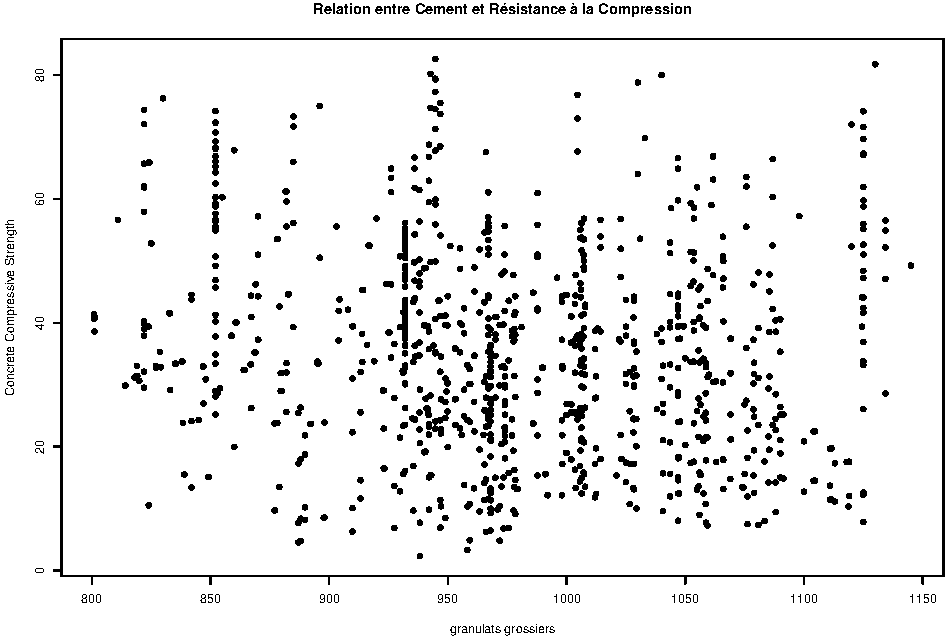
\includegraphics{rmd_final_files/figure-latex/unnamed-chunk-13-1} \end{center}

\subsubsection{Partie E}\label{partie-e}

\begin{Shaded}
\begin{Highlighting}[]
\CommentTok{\# Représentation des variables sur le plan factoriel (axes 1 et 3)}
\FunctionTok{plot.PCA}\NormalTok{(}
\NormalTok{  res\_pca,}
  \AttributeTok{axes =} \FunctionTok{c}\NormalTok{(}\DecValTok{1}\NormalTok{, }\DecValTok{3}\NormalTok{),             }\CommentTok{\# On se concentre sur les 2 premiers axes}
  \AttributeTok{choix =} \StringTok{"var"}\NormalTok{,              }\CommentTok{\# Afficher les variables dans le plan factoriel}
  \AttributeTok{col.var =} \StringTok{"\#4B0000"}\NormalTok{,        }\CommentTok{\# Couleur des variables alignée au style}
  \AttributeTok{col.quanti.sup =} \StringTok{"\#0000FF"}\NormalTok{, }\CommentTok{\# Couleur pour la variable quantitative supplémentaire}
  \AttributeTok{label =} \StringTok{"all"}\NormalTok{,}
  \AttributeTok{title =} \StringTok{""}\NormalTok{,}
  \AttributeTok{addgrid.col =} \StringTok{"\#DDB688"}     \CommentTok{\# Couleur de la grille}
\NormalTok{)}
\end{Highlighting}
\end{Shaded}

\begin{center}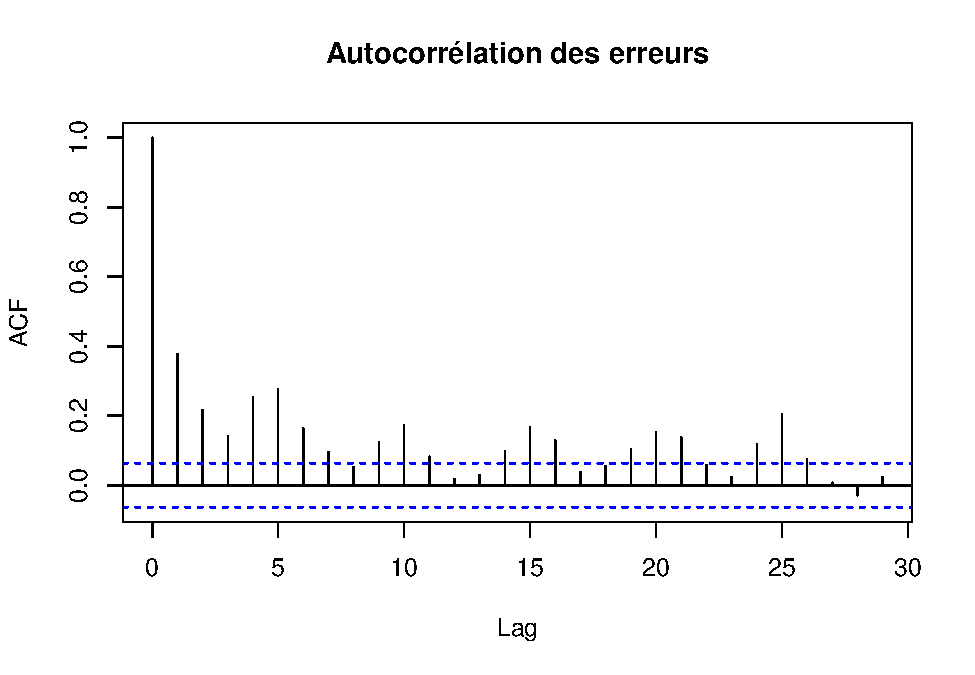
\includegraphics{rmd_final_files/figure-latex/unnamed-chunk-14-1} \end{center}

\end{document}
